\documentclass{article}
\usepackage[margin=1in]{geometry}
\usepackage{amsmath}
\usepackage{amsfonts}
\usepackage{graphicx}
\usepackage{blindtext}
\usepackage{hyperref}

\hypersetup{
    colorlinks=true,
    linkcolor=blue,
    filecolor=magenta,      
    urlcolor=cyan,
}

%\title{Project Proposal \\ CS 395 - Deep Learning}
%\author{Adam Barson, Daniel Berenberg}
\begin{document}
\begin{titlepage}
    \begin{center}
        \vspace*{8cm}
        
        {\Large\textbf{Predicting User Heart Rate with Action Recognition}}
        
        \vspace{0.5cm}
        
        \textbf{Adam Barson \& Daniel Berenberg}
        
        \vspace{0.5cm}
        CS 395 - Deep Learning \\
        University of Vermont \\
        
    \end{center}
\end{titlepage}

\section*{Introduction}{Millions of Americans are afflicted with panic disorder, a psychiatric disorder in which debilitating fear and anxiety arise with no apparent cause. There are several clinically available methods to treat panic disorder, many of which involve either medication or intensive psychotherapy. One simple therapeutic tactic that has been shown to help control the symptoms of recurring panic attacks and to mitigate the risk of future attacks is to show a patient suffering from a panic attack their heart rate and respiratory rate. The ability of panic disorder sufferers to have access to their heart rate and respiratory rate at any given time, therefore, would be quite beneficial to the long-term management of the disorder.  \\ \\
\noindent To make this treatment method as accessible as possible to every panic disorder sufferer, a solution is being explored that would make use of the ubiquitous smartphone. There is promising evidence to suggest that pulse is detectable by smartphone cameras: one can lightly press their finger up to a smartphone camera with flash on, and produce a video that clearly shows their pulse. This project aims to leverage deep learning techniques to predict a patient?s heart rate, given short videos of this nature.}
%%%%%%%%%%%%%%%%%%%%%%%%%%%%%%%%%%%%%%%%%%%%%%%%%%%%%%%%%%%%%%%%%%%%%%
\section*{Problem Definition and Algorithm}{The dataset used by this project has been provided by Dr. Ryan McGinnis of the University of Vermont Biomedical Engineering department. Video data was collected from 31 subjects, where each patient recorded their finger lightly placed on, but entirely covering, a smartphone camera. Two videos were recorded of each subject-- one at a resting heart rate, and one after an intense 60 second workout. All videos gathered during the study are around 30 seconds long. The heart rate and respiratory rate for each subject were also recorded and provided along with the video data. The aim of this project is to train a deep neural network on this labeled video data to accurately predict heart rate and respiratory rate given a short video of a finger pressed up to a smartphone camera. \\ \\
\noindent We have decided to implement a variety of action detection models for our project. Thus far, we have trained two classifiers, which are being used to differentiate between ?high? and ?low? heart rates. We go into more detail in the section below. The ultimate goal of the project is to train a regression model that, instead of simply performing binary classification, will actually output a heart rate and respiratory rate, given a video input. }
%%%%%%%%%%%%%%%%%%%%%%%%%%%%%%%%%%%%%%%%%%%%%%%%%%%%%%%%%%%%%%%%%%%%%%
\section*{Experimental Evaluation}{
The preliminary experiment conducted was an attempt to train a binary classification model from scratch that would accurately determine whether a video showed a  ``high'' or ``low'' heart rate, where a ``high'' heart rate is defined as any heart rate that is greater than 100 beats per minute and a ``low'' heart rate is defined as any heart rate that is not considered ``high''. \\ \\
\noindent There are at least two reasons why the first step to our problem entails a binary classifier. First, we want to affirm that processing and differentiating the samples in our dataset is indeed feasible. Second, the binary classifier may prove useful as part of the input to the subsequent regression model. Hence, creating the binary classifier serves to both prove a hypothesis and function as a parameter of interest later in the project. \\ \\
\noindent The hypothesis that we would like to test in this experiment is that the data serves as a valuable, valid input to our problem and that the means by which we preprocessed the data were in fact useful and not detrimental to our ultimate goal.
\subsection*{Methods}{The preliminary experimentation for the project was broken into three stages: \textit{preprocessing}, \textit{training/testing}, and \textit{results}.
\subsubsection*{Preprocessing}{This stage consisted of creating a suite of python and shell scripts that organized, standardized, resized, and partitioned the data. Since the original data format started with was \textit{.mov}, the first step was to separate each video file into a sequence of frames. Afterwards, each sequence of frames was tested whether it was drawn from a video of 30 frames per second or 60 frames per second. Sequences deemed to be 60 frames per second were down sampled to 30 frames per second. Finally, the size of each frames in each sequence was transformed from $(1920 \times 1080 \times 3)$ to $(224 \times 224 \times 3)$. The data now existed as a set of 62 approximately 900 $(224 \times 224 \times 3)$ frame sequences. The final step was to take prescribed ``good'' samples and partition each of their 900 frames into separate sequences of 60 frames, or two seconds of video. We then organized the data into a directory structure conducive for the needs of easy access during training and generated a \textit{.csv} file that catalogued the position and labels (heart rate, respiratory rate) of each sample.
}}
\subsubsection*{Training/Testing}{After the preprocessing stage, the next step was to create classification models that could attempt the task at hand. Through online tutorials, github sources, and journal articles, we each created a separate architecture and trained it. Each model architecture is seen below. \\

%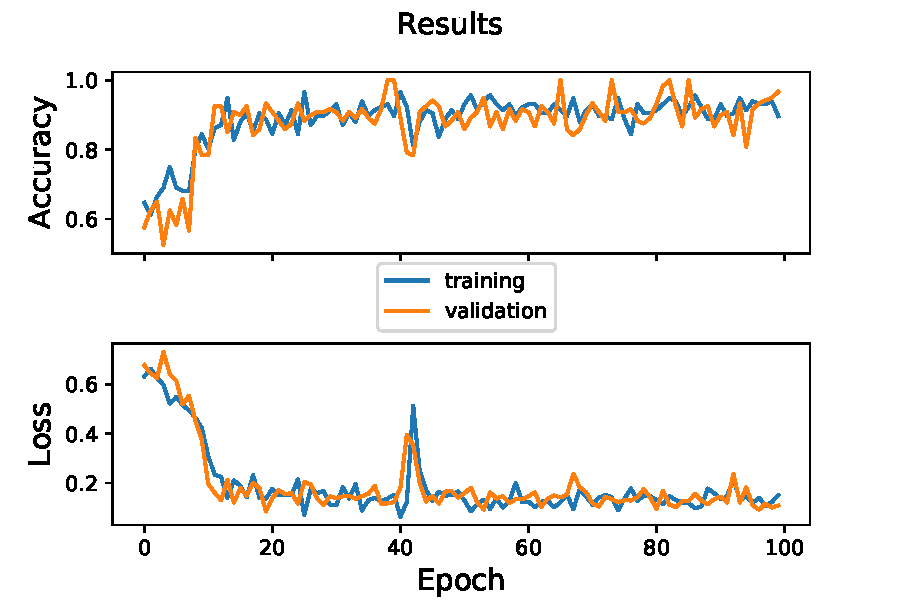
\includegraphics{../figs/midway_results.pdf}\includegraphics[width=0.6\textwidth]
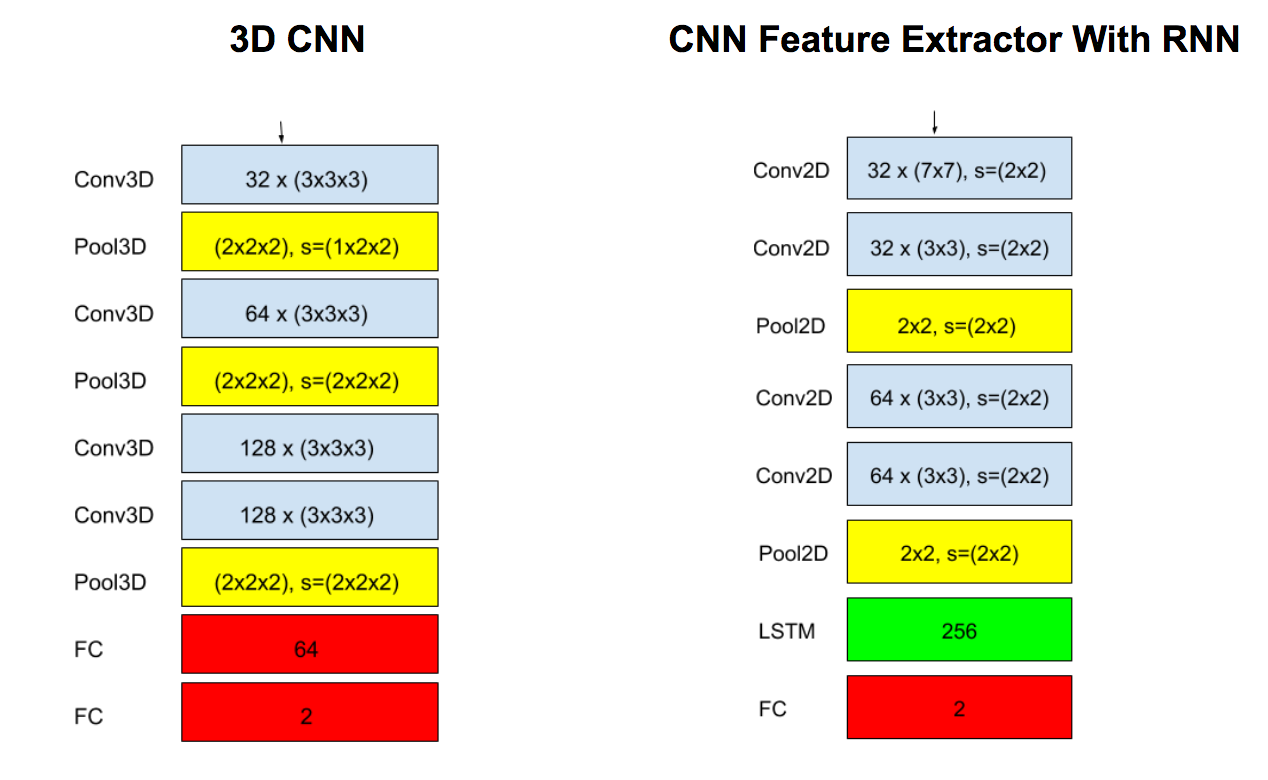
\includegraphics[width=0.9\textwidth]{../figs/models.png} \\
%
\noindent The left model is a 3D CNN that simply consists of several 3D convolutional and max pooling layers, followed by a 64-neuron fully connected layer and an output to two classes. The right model is a traditional CNN with an RNN (LSTM) concatenated to the end. The RNN outputs one of the two classes ``high'' or ``low''.  \\ \\
\noindent From the preprocessing stage, 147 good partitions and their corresponding labels were generated. This set of 60 frame partitions was broken into a training set of 117 samples and a testing set of 30 samples. The models were trained and tested, the results of which are discussed in \textit{Results}.}
\newpage
\subsubsection*{Results}{
Shown below is the loss and accuracy results from training the LSTM + CNN model for 100 epochs and testing it on each training epoch. \\
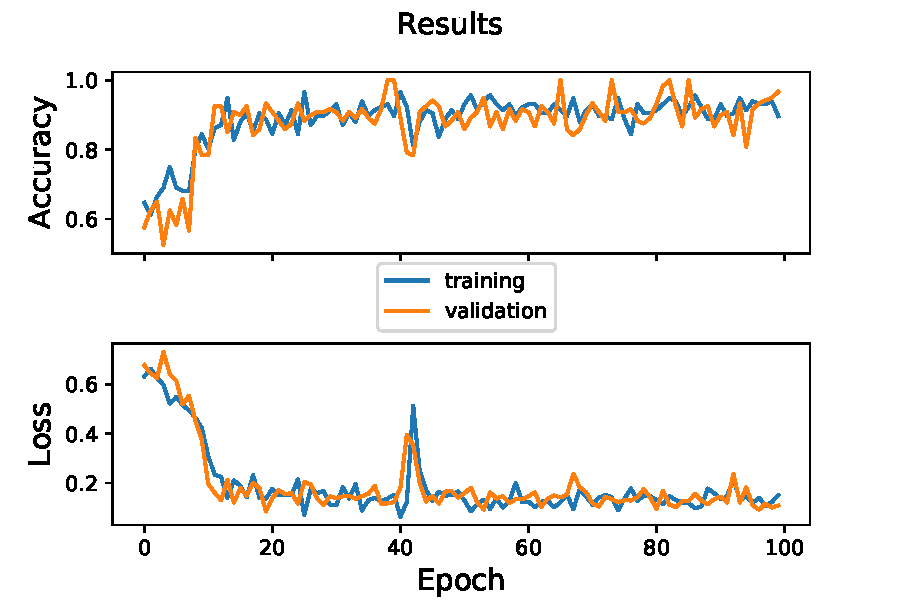
\includegraphics{../figs/midway_results.pdf} \\
The plot above shows that the model is quite successful in accurately predicting the class of a given video clip. We were a bit suspicious of these results, the reason for which is described in the Issues section. Our explanation for this performance is that the data, unlike most video datasets, is highly homogenous; the each partition sequence is a mostly red-hued set of frames with low variability per frame. This allow the CNN to determine more complex features of the data that differentiate the ``high'' and ``low'' classes without having to worry about the pixel variance per frame traditionally common in video data.
}}
%%%%%%%%%%%%%%%%%%%%%%%%%%%%%%%%%%%%%%%%%%%%%%%%%%%%%%%%%%%%%%%%%%%%%%
\section*{Related Work}{There are a multitude of related projects on GitHub that we have been using as inspiration for our project. \\

\noindent \href{https://github.com/harvitronix/five-video-classification-methods/blob/master/train_cnn.py}{This} git repository showcases five different methods for using keras and tensorflow in video classification problems. In particular, we are interested in the model that reportedly produced the best results: a CNN feature extractor, combined with a RNN. The RNN is connected to a dense 2 neuron softmax layer, which is the output of the model. The model provided in this repository was a bit heavy for our needs (it contains several more million parameters than our model), so we repurposed the model to contain fewers layers, and fewer overall trainable parameters. \\ }
%%%%%%%%%%%%%%%%%%%%%%%%%%%%%%%%%%%%%%%%%%%%%%%%%%%%%%%%%%%%%%%%%%%%%%
\newpage
\section*{Next Steps}{
\subsection*{Issues}{We have achieved very promising results so far in our classification attempts. Before moving on to the final stages of the project, however, there are a few important issues that we must address.
\subsubsection*{Data Size}{Naturally, given the small size of our data set, we face some limitations in training a robust network. Our next steps, therefore, will primarily be directed at obtaining more data, via having subjects record more videos, and data augmentation. Data augmentation will consist of choosing some set of random modifications to make on 60 frame sequences during training. We hope that using data augmentation will help us both fight overfitting and train a more generalizable network.}
\subsubsection*{Training/Testing Selection}{Another issue that we have faced so far is in regard to how our training and testing data is selected. After preprocessing the video data, we were left with 147 60-frame sequences. Each subject has around 24 sequences that belong to them, half of which come from the resting heart rate recording, and the other half of which come from the recording that took place following an intense 60 second workout. In training our network, we split up these 147 sequences into training and testing sets, which come out to a 117/30 training/testing split. At the moment, our data splitting method has no way of ensuring that the training data and testing data sets do not contain sequences that belong to the same subject. In short, it is possible that the reported accuracy of our model may not reflect how well the model actually generalizes, due the model potentially training and testing on different sequences of the same subject. This is problematic due to the fact that while two different sequences belonging to the same subject are not exactly the same, they tend to be very similar. A more nuanced selection of training and testing sets may be called for to address this potential problem. Data augmentation is also a way in which we may further mitigate this issue. The severity of this data selection problem will be assessed by testing the model on several subjects that it has not yet been exposed to.
}
\subsubsection*{Other Models}{While our CNN + LSTM classifier so far has yielded very promising results, we hope to explore more potential models to see if we can achieve even better classification accuracy. We believe that by first training a classifier that is as accurate as possible, we will have better chances in successfully training a regression model.}}
\subsection*{Timeline}{After addressing these aforementioned issues, we will begin training a regression model. The regression model will be an extension of the classifier that performed the best. We believe that our goal of successfully training a regression model is doable, given the timeline below:
\begin{itemize}
\item[3/26]{Implement data augmentation}
\item[3/31]{Implement a more scrupulous data splitting process}
\item[4/01]{Train the most optimal classifier possible}
\item[4/10]{Train a regression model}
\item[4/17]{Enhance regression model}
\end{itemize}}
}
\section*{Code \& Dataset}
{Our dataset is confidential and was distributed to us through UVM Biomedical Engineering. The code can be found by following this link: \href{https://github.com/danielberenberg/DeepLearning-BloodData}{https://github.com/danielberenberg/DeepLearning-BloodData}. o reproduce the results described in this report the user should do the following:
\begin{enumerate}
\item{Obtain access to confidential dataset, including the \textit{.csv} files \texttt{DeepLearningClassData.csv} and \texttt{GoodStartingPoint.csv}.}
\item{Run \texttt{preprocess.sh} found in the \texttt{scripts} directory.}
\item{Run the command \texttt{python scripts/trainer.py consolidated/ partitions\_cons.csv}, this will train a network from scratch and save high performing models to a directory called \texttt{models}.}
\end{enumerate}
The scripts called in \texttt{preprocess.sh} format and organize the data into a directory that the training script can easily access and select data from. 
}
\section*{Conclusion}
{We have proven that deep learning techniques work well in classifying our data set, as a 90\% test accuracy was achieved by using a CNN + LSTM model to classify between low and high heart rates. Several adjustments will be made to our methodologies, which will enhance further training of the model, and allow testing that more accurately reflects the performance of the model. \\ \\
\noindent Before we move forward and attempt to train a regression model, some preliminary steps must be taken first. Namely, issues involving a lack of data and possible issues surrounding the manner in which training and testing data are selected must be addressed to ensure that we train the most accurate regression model possible.}
 \newpage
 \section*{Citations}
 {[1] Harvey, M. (2017, March 22). Five video classification methods implemented in Keras and TensorFlow. Retrieved March 21, 2018, from https://blog.coast.ai/five-video-classification-methods-implemented-in-keras-and-tensorflow-99cad29cc0b5 \\ \\

\noindent[2] Ng, J. Y., Hausknecht, M., Vijayanarasimhan, S., Vinyals, O., Monga, R., \& Toderici, G. (2015). Beyond short snippets: Deep networks for video classification. 2015 IEEE Conference on Computer Vision and Pattern Recognition (CVPR). doi:10.1109/cvpr.2015.7299101
}
\end{document}